\documentclass[12pt,twoside]{article}
\usepackage{amsmath, amssymb}
\usepackage{amsmath}
\usepackage[active]{srcltx}
\usepackage{amssymb}
\usepackage{amscd}
\usepackage{makeidx}
\usepackage{amsthm}
\usepackage{algpseudocode}
\usepackage{algorithm}
\usepackage{graphicx}
\usepackage[spanish]{babel}
\renewcommand{\baselinestretch}{1}
\graphicspath{{images/}}
\setcounter{page}{1}
\setlength{\textheight}{21.6cm}
\setlength{\textwidth}{14cm}
\setlength{\oddsidemargin}{1cm}
\setlength{\evensidemargin}{1cm}
\pagestyle{myheadings}
\thispagestyle{empty}
\markboth{\small{Pr\'actica 4. Alan, Josu\'e}}{\small{.}}
\date{}
\begin{document}
\centerline{\bf An\'alisis de Algoritmos, Sem: 2020-1, 3CV2, Pr\'actica 4, 28 de agosto}
\centerline{}
\centerline{}
\begin{center}
\Large{\textsc{Pr\'actica 4. Divide y vencer\'as, algoritmo QuickSort}}
\end{center}
\centerline{\bf{Alan Romero Lucero, Josu\'e David Hern\'andez Ram\'irez}}
\centerline{}
\centerline{Escuela Superior de C\'omputo}
\centerline{Instituto Polit\'ecnico Nacional, M\'exico}
\centerline{$alanrl.escom@gmail.com, correo@alumno_2$}
\newtheorem{Theorem}{\quad Theorem}[section]
\newtheorem{Definition}[Theorem]{\quad Definition}
\newtheorem{Corollary}[Theorem]{\quad Corollary}
\newtheorem{Lemma}[Theorem]{\quad Lemma}
\newtheorem{Example}[Theorem]{\quad Example}
\bigskip
\textbf{Resumen:} Con esta pr\'actica se pretende analizar otra manera de utilizar el principio divide y vencer\'as, esta vez con el algoritmo \textit{QuickSort}.
{\bf Palabras Clave:} {\textit{algoritmo, ordenamiento, $big O$, quick sort, pivote}}
\section{Introducci\'on}
Existe una cantidad enorme de algoritmos de ordenamiento, cada uno reconocido con un nombre, dependiendo del algoritmo que se utiliza que tiene alguna car\'acter\'istica especial que los hace f\'acilmente reconocibles. Por ejemplo, el algoritmo burbuja, el \textit{MergeSort}, \textit{InsertionSort}, etc. Pero de entre todos, hay un algoritmo que presume de ser \textit{"r\'apido"}, este es el famoso \textit{QuickSort}, pero, ¿Qu\'e tan complejo es? ¿Es realmente r\'apido para todos los casos? ¿Por qu\'e funciona tan bien? Bueno pues, como se podr\'ia esperar, el algoritmo utiliza la conocida t\'ecnica de \textit{divide y vencer\'as}, pero hace falta analizarlo m\'as a fondo y entender mejor su funcionamiento.

\section{Conceptos B\'asicos}
El \textit{QuckSort} trabajo bajo el principio b\'asico de divide y vencer\'as. tal como lo hace el \textit{MergeSort} solo que implementado de otra manera. Ahora, ve\'ase el pseudo-c\'odigo de este algoritmo
\begin{center}[ht]
    \begin{algorithmic}[1]
        \Procedure{QuickSort}{n=$[A\textsubscript{1}, \dots, A\textsubscript{len}]$, p, r}
            \If{$p < r$}
                \State $q \longleftarrow \textbf{partition}(n, q, r)$
                \State \textbf{QuickSort}(n, p, q - 1)
                \State \textbf{QuickSort}(n, q + 1, r)
            \EndIf
        \EndProcedure
    \end{algorithmic}
\end{center}
Resulta que, de manera an\'aloga al ya mencionado \textit{MergeSort}, hay un algoritmo clave en el \textit{QuickSort} que hace que todo funciona, el algoritmo de la funci\'on \textit{partition}. A continuaci\'on el algoritmo mencionado.
\begin{center}
    \begin{algorithmic}[1]
        \Procedure{partition}{n = $[n\textsubscript{1},\dots,n\textsubscript{n}]$, q, r}
            \State $x \longleftarrow n[r]$
            \State $i \longleftarrow p$
            \For{$j \text{ from } p \text{ to } r$}
                \If{$n\textsubscript{j} < x$}
                    \State \textbf{exchange}($n\textsubscript{i}$, $n\textsubscript{j}$)
                    \State $i \longleftarrow i + 1$
                \EndIf
            \EndFor
            \State \textbf{exchange}($n\textsubscript{i}$, $n\textsubscript{j}$)
            \State \textbf{return} $i$
        \EndProcedure
    \end{algorithmic}
\end{center}
En el algoritmo anterior se hace un "\textit{exchange}", es decir, se intercambian los valores que se pasan en el arreglo. Esta funci\'on toma un \textit{pivote}, desde el cual se divide al arreglo en dos partes las cuales estar\'an divididas por el pivote y mediante intercambios se estar\'an pasando elementos de un lado a otro hasta que los menores y mayores quedaran separados. Si se hace esta partici\'on con arreglos cada vez mas pequeños, como lo hace le \textit{QuickSort} al final los arreglos terminaran completamente ordenados. De esta forma, el problema fue dividido en pequeño problemas, ya que el algoritmo \textit{partition} es de complejidad lineal.

Analizando por bloque el c\'odigo para hacer la partici\'on, resulta evidente que en el cuerpo del for solo existen bloques de complejidad constante $\Theta(1)$. El for es complejidad $\Theta(n)$ y a parte, las dem'as lineas son de complejidad constante, por lo que su complejidad seria $\textbf{partition} \in \Theta(n)$.

Por otro lado, el \textit{QuickSort} es recursivo por lo que hace falta una ecuaci\'on de recurrencia. Esto es especial en este algoritmo, debido a que el pivote es variable y no sabemos bien como se comportara. La siguiente ecuaci\'on se plantea cuando el elemento pivote se encuentra en los extremos, dado que es el pero caso.
\[
    T(n) = 
\begin{cases}
    c, & \text{si } n \leq 1 \\
    T(1) + T(n-1) + cn, & n > 1
\end{cases}
\]

Resolviendo esta ecuaci\'on de recurrencia se llega a lo siguiente
\begin{figure}[ht]
    \centering
    \begin{equation}
        \dots = c + cn + c(n-1) + \dots + T(1)
    \end{equation}
    \begin{equation}
        \text{Mediante una sumatoria}
    \end{equation}
    \begin{equation}
        T(n) = (n-1)c + \frac{n(n+1)}{2}
    \end{equation}
    \caption{Ecuaci\'on de recurrencia reducida}
    \label{eq:ecuacion_recurrencia}
\end{figure}

Por lo que llega a una complejidad cuadr\'atica en el peor de los caos. Cuando el pivote divide al arreglo por la mitad, se comporta como el \textit{MergeSort} de la pr\'actica anterior, con ecuaci\'on de recurrencia: 

\[
    T\textsubscript{1}(n) = 
\begin{cases}
    c, & \text{si } n \leq 1 \\
    2T(\frac{n}{2}) + bn, & n > 1
\end{cases}
\]

Adem\'as es un caso promedio, por lo que se tiene que $T(n) \in \mathcal{O}(n^2)$ y $T\textsubscript{1}(n) \in \Theta(n\log_2 n)$.

\newpage
\vfill
\clearpage

\section{Experimentaci\'on y Resultados}
La implementaci\'on de los algoritmos se hizo de manera aleatoria, sin embargo, se agrego la opci\'on para su ejecuci\'on en el peor de los casos. Dada la manera en que funciona el \textit{MergeSort}, las gr\'aficas generadas con valores aleatorios es bastante, valga la redundancia, aleatoria. Por ejemplo, con el algoritmo \textit{partition} la complejidad se ve claramente limitada con su complejidad lineal. Sin embargo, con el algoritmo del \textit{QuickSort} la complejidad se ve bastante reducida, debido evidentemente a que su complejidad promedio es bastante bajo.
En cambio, cuando se encuentran los peores casos las gr\'aficas son mas claras.

\begin{figure}{h}
    \centering
    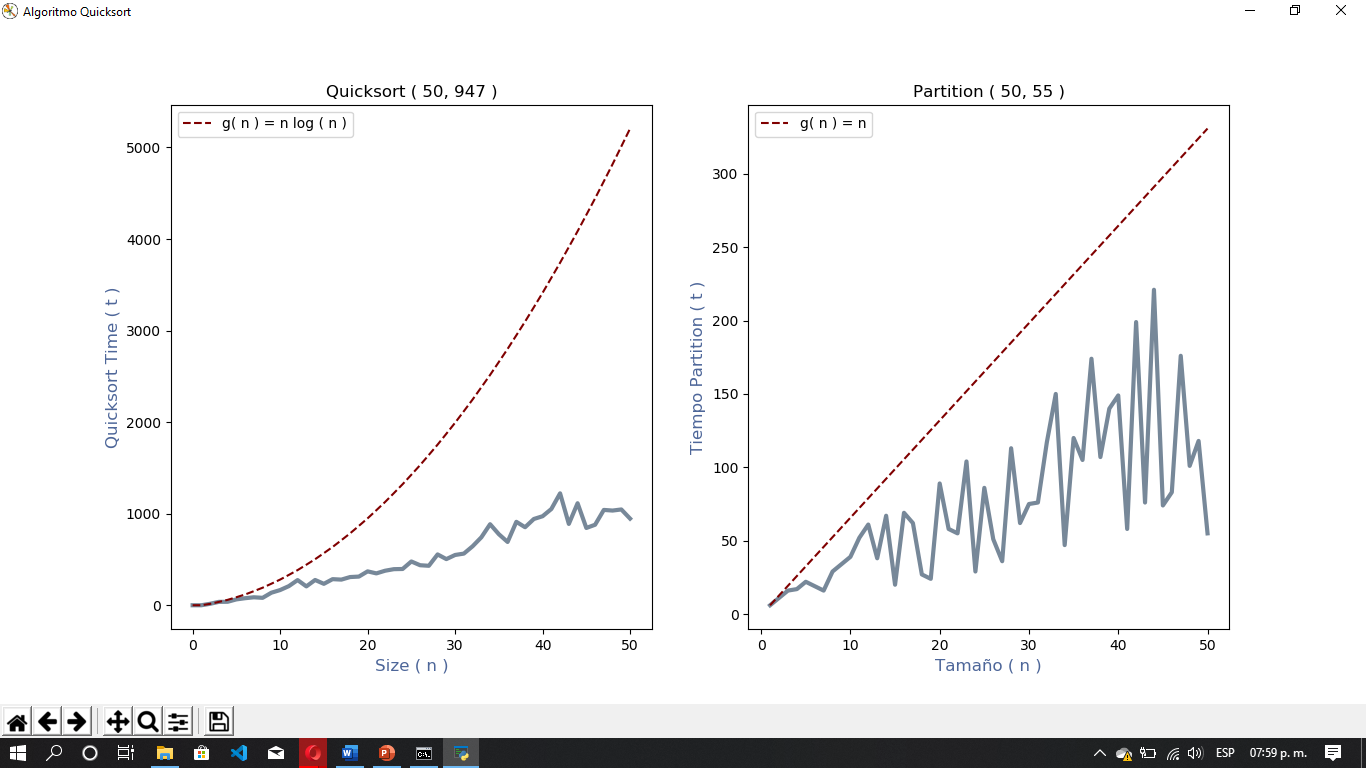
\includegraphics[width=13cm, height=6cm]{quick_graph.png}
    \caption{Gr\'afica del algoritmo QuickSort y parition, con variables aleatorias }
    \label{fig:quick_graph}
\end{figure}

\begin{figure}{h}
    \centering
    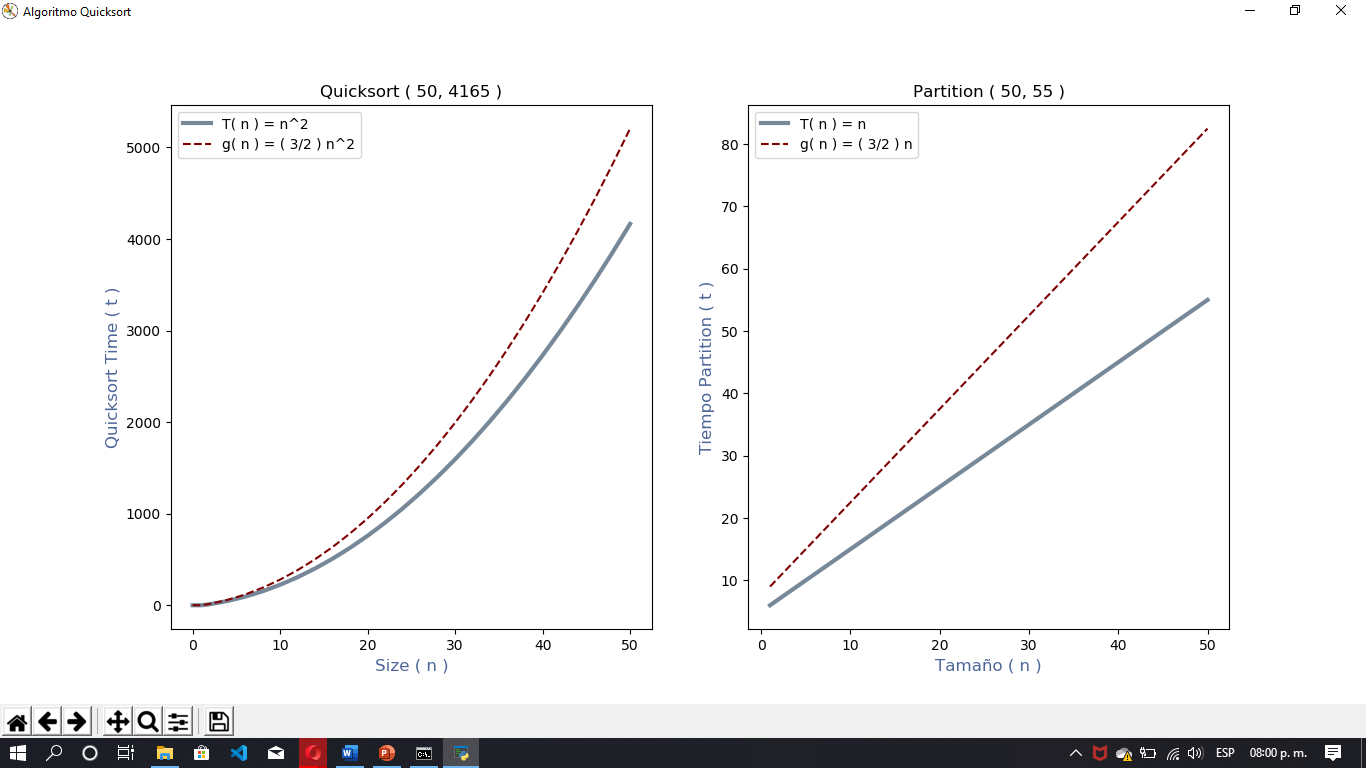
\includegraphics[width=13cm, height=6cm]{quick_worst.png}
    \caption{Gr\'afica del algoritmo QuickSort y parition, en el pero de los casos }
    \label{fig:quick_worst}
\end{figure}

\begin{figure}{h}
    \centering
    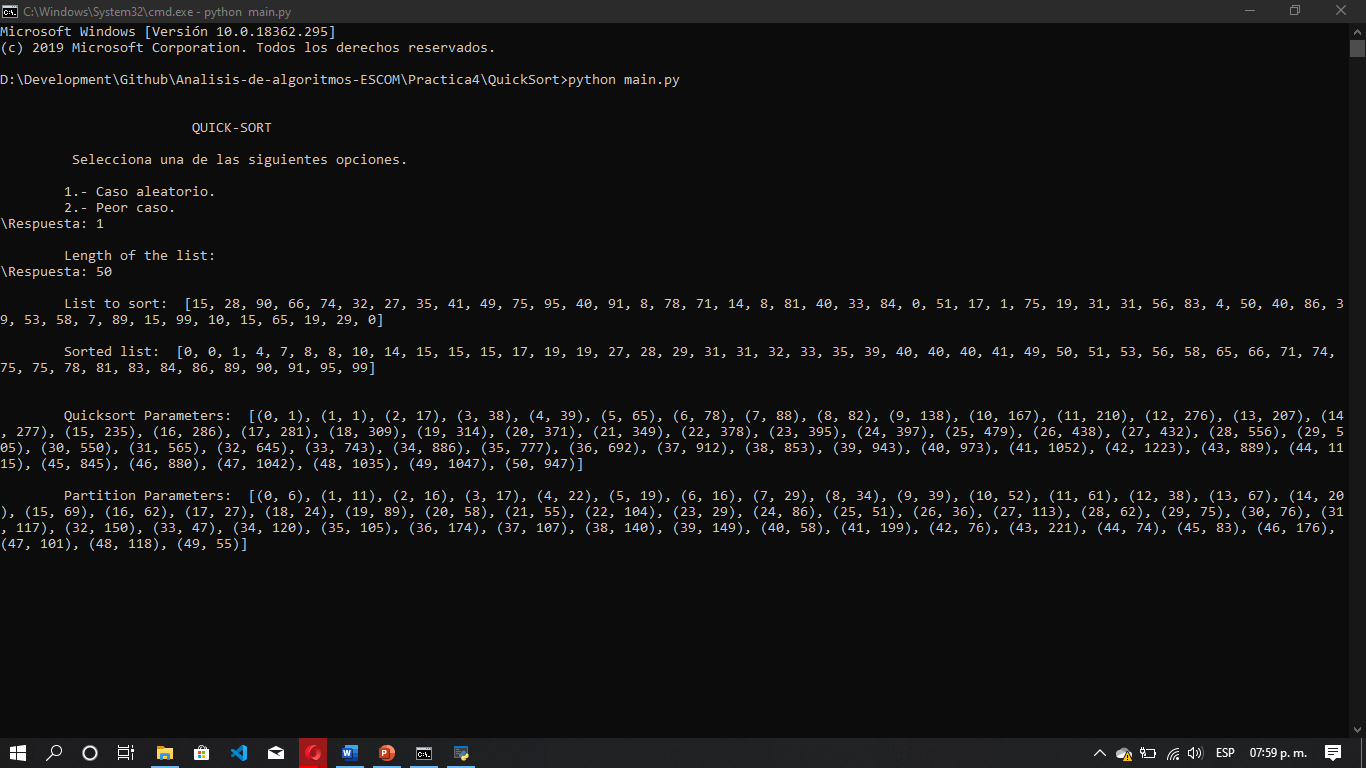
\includegraphics[width=13cm, height=6cm]{quick_prog.png}
    \caption{Programa del QuickSort y Partition en ejecuci\'on}
    \label{fig:quick_program}
\end{figure}


\section{Conclusiones}

\textit{Alan Romero Lucero}. El funcionamiento del \textit{QuickSort} es interesante de analizar. A pesar de ser llamado "quick", aparentemente el MergeSort tiene menor complejidad en el peor de los casos, aunque depende mucho del caso debido a que seg\'un el pivote puede tener tambi\'en bastante buen tiempo de ejecuci\'on. Independientemente de esto, es clara la importancia de dividir el problema, como con el MergeSort, para reducir la complejidad y tener problemas mas simples por resolver.


\\\\\textit{Josu\'e David Hern\'andez Ram\'irez}. Como hemos visto en clase y lo hemos comprobado de manera gr\'afica, estos algoritmos regularmente tienen complejidad $\Theta(n\log_2 n)$ pero en casos cr\'iticos tiene complejidad $\Theta(n^2)$ esto se debe a la elección de la posición del pivote el cual podemos controlar para que su complejidad disminuya y por ende, sea más eficiente que el algoritmo visto anteriormente\textit{mergesort}.

Con puedo comprobar que entre mas se divida el problema mejores resultados obtendr\'e respecto al tiempo de resoluci\'on.
 
\newpage
\vfill
\clearpage
\section{Anexo}
¿Qu\'e valor de q retorna Partition cuando todos los elementos en el arreglo A[p, ..., r]
tienen el mismo valor?
Dado que recorre todos los elementos y nunca ocurre la condici\'on de que un elemento sea estrictamente menor que otro, dado que valen lo mismo, siempre regresara el indice inicial p.

¿Cu\'al es el tiempo de ejecuci\'on de QuickSort cuando todos los elementos del arreglo
tienen el mismo valor?
Como se analizo en la pregunta anterior, debido a que la partici\'on siempre regresara el \'indice de los extremos, se encuentra en el peor caso del \textit{QuickSort}, por lo que pertenece a $\mathcal{O}(n^2)$.

\section{Bibliograf\'ia}
"QuickSort", class notes for An\'alisis de Algoritmos, ESCOM-IPN, Verano 2019.
\end{document}